\chapter{Encryption schemes with integrity guarantees}

\section{IND-CCA2 Authenticated Encryption}

\begin{flushleft}
    La crittografia ``normale'' deve rispettare il requisito di \textbf{confidenzialità} contro un modello di attaccante del tipo \textbf{CPA} e \textbf{CCA1}. Per quanto riguardo la modellazione \textbf{CCA2} per riuscire a garantirne confidenzialità è necessario aggiungerci anche garanzie di \textbf{integrità} (tramite le \textit{hash funciton}) e \textbf{autenticità} (tramite \textit{MAC}). Chiameremo \textbf{\textit{Authenticated Encryption}} questi schemi crittografici che garantiscono \textbf{confidenzialità}, \textbf{integrità} e \textbf{autenticità}. In casi di utilizzo reale:
    \begin{itemize}[nosep]
        \item utilizzare schemi standard che garantiscono tutti questi requisiti.
        \item se non fossero disponibili, bisogna costruirsene uno partendo da uno schema non autenticato e da un MAC.
    \end{itemize}

    In maniera generale per riuscire ad ottenere \textit{authenticated encryption} sono necessarie due primite che verranno utilizzate a \textit{black-box}: \textit{block cipher} e \textit{MAC scheme}. È possibile combinare questi tre elementi in tre maniere differenti.

    {\centering
        \begin{minipage}[c]{0.30\textwidth}
            \centering
            \textbf{\textit{Encrypt-and-MAC}} \\
            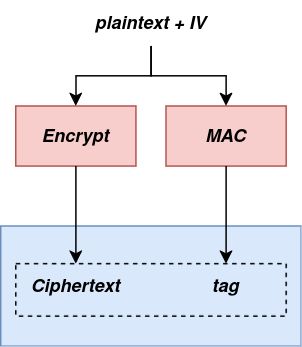
\includegraphics[width=0.75\textwidth]{img/enc_and_mac.png}
            
            In questo caso viene cifrato il testo in chiaro e composto il MAC in maniera parallela e poi vengono concatenati i risultati. Non ho alcuna garanzia che garantisca la confidenzialità del messaggio.

        \end{minipage}
        \begin{minipage}[c]{0.30\textwidth}
            \centering
            \textbf{\textit{MAC-then-Encrypt}} \\
            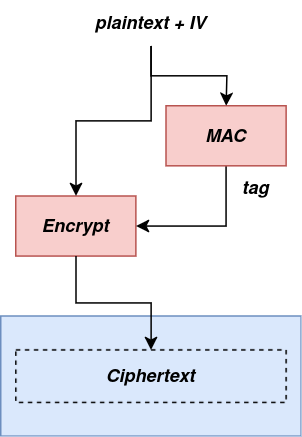
\includegraphics[width=0.75\textwidth]{img/mac_then_enc.png}

            Prima calcola il \textit{tag} e poi cifra la concateazione tra \textit{tag} e \textit{plaintext}.

        \end{minipage}
        \begin{minipage}[c]{0.30\textwidth}
            \centering
            \textbf{\textit{Encrypt-then-MAC}} \\
            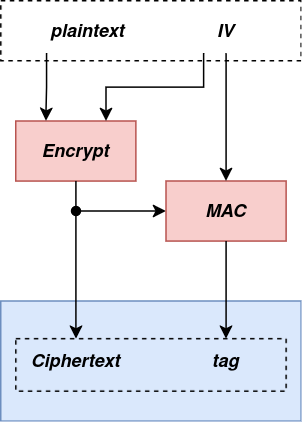
\includegraphics[width=0.75\textwidth]{img/enc_then_mac.png}

            Prima si calcola il crittogramma che poi verrà utilizzato per generare il \textit{tag}, concatenando in seguito il risultato. Il MAC è calcolato sul testo cifrato quindi non è possibile informazioni aggiuntive

        \end{minipage}
    \par}

    Considerando tutti e tre le combinazioni degli schema l'unica che garantisce il rispetto dei requisiti di sicurezza anche senza considerare le primitive sottostantei è l'\textbf{\textit{encrypt-then-MAC}}.
    \begin{enumerate}[nosep]
        \item la funzione \textbf{MAC} deve autenticare non solo il testo cifrato, ma anche l'IV.
        \item lo schema di crittografia e la funzione di MAC devono utilizzare due tipologie di \textbf{chiavi differenti}.
        \item nella fase di \textit{decryption} il \textbf{tag} deve essere verificato \textbf{prima} di iniziare la decifratura in quanto un'attaccante potrebbe mettere in pratica un \textbf{\textit{timing attack}}, ovvero ottenere informazioni dal tempo di esecuzione di una certa funzione.
    \end{enumerate}
    Un'altra cosa fondamentale è che le funzioni crittografiche (\textit{encryption} e \textit{decryption}) devono essere \textbf{\textit{time-constant}}
\end{flushleft}

\newpage

\begin{flushleft}
    \textcolor{red}{\textbf{\textit{Authenticated Encryption with Associated Data - AEAD}}}
    \begin{lstlisting}
    key = keygen([size])
    cipher = encrypt(key, nonce/iv, a, plain)
    plain = decrypt(key, nonce/iv, a, cipher)
    \end{lstlisting}
    \vspace*{-\baselineskip}
    I \textbf{dati associati} non sono cifrati né inclusi nel crittogramma (principalmente per vincoli definiti dal contesto in cui sono), ma l'autenticità è invece vincolata anche a quell'informazione. In questo modo l'operazione di decifratura verificherà che gli \textit{associated data} siano gli stessi dell'\textit{encryption}, in caso contrario, \textbf{fallirà} riuscendo a garantire:
    \begin{itemize}[nosep]
        \item confidenzialità, autenticità e integrità del \textit{plaintext}.
        \item autenticità e integrità dei dati associati.
    \end{itemize}
    Aggiungono \textit{overhead} sia a livello computazine che di \textit{storage}.
\end{flushleft}

\section{IND-CCA1 Encryption Schemes \\ \small{length-preserving scheme for disk encryption}}

\begin{flushleft}
    Non è possibile garantire forte autenticità (CCA2) senza adottare l'uso di MAC, ma in questo modo uno schema \textit{CCA2 secure} introdurrà dell'\textit{space overhead} rispetto a schemi non autenticati. In certi scenari è preferibile - se non richiesto - che il testo cifrato abbia la \textbf{stessa dimensione} del \textit{plaintext}, molti di questi scenari sono i \textbf{\textit{disk (sector) encryption}}. In questi scenari la migliore sicurezza che riusciamo a garantire è \textbf{IND-CCA1}.

    \smallskip

    Per come si è descritto lo scenario un \textit{stream cipher} - che per definizione è completamente \textbf{malleabile} - è la peggior progettazione possibile in quanto non possiamo autenticare (in quanto introducerebbe un \textit{overhead}), è quindi guidata la scelta verso i \textit{block cipher} - storicamente è sempre stato preferito il \textit{mode of operations} \textbf{CBC}. I problemi di \textbf{CBC} legati ad attacchi attivi sono:
    \begin{itemize}[nosep]
        \item molto vulnerabili contro la \textbf{manipolazione dell'\textit{IV}}.
        \item molto vulnerabili contro attacchi del tipo \textbf{\textit{ciphertext substitutions}} (es. \textit{efail}).
        \item il \textit{padding} può aiutare l'attaccante.
        \item ``\textit{functional issue}'': i blocchi sono \textbf{interdipendenti}.
    \end{itemize}

    \smallskip

    Per la cifratura del disco ci sono alcuni requisiti che vanno rispettati, tra cui: la lunghezza del testo cifrato deve essere uguale al testo in chiaro (nessun \textit{IV} o \textit{nonce} e nessun \textit{tag}), livello di sicurezza contro \textbf{attacchi CCA1} (è impossibile per l'attaccante avere un riscontro di cosa è stato modificate - scenario non adattivo) e ultimo, ma non per importanza è che devono essere veloci. Da questo possiamo andare a definire cosa alcune intuizioni di progettazione:
    \begin{itemize}[nosep]
        \item la crittografia deve essere a \textbf{blocchi}.
        \item i blocchi devono essere \textbf{indipendenti} uno dall'altro, ma comunque non malleabili (\textbf{no CTR}) e random (\textbf{no ECB}).
        \item la randomicità non deve però introdurre problematiche di malleabilità e deve essere indipendente da ogni blocco (\textbf{no CBC-IV} con effetto a valanga).
        \item è possibile utilizzare i \textbf{\textit{sector number}} - anche noti come \textbf{\textit{tweaks}} - al posto del nonce.
    \end{itemize}
    Ricordiamoci che la garanzia di sicurezza richiesta da questo scenario è \textbf{\textit{CCA1 secure}}, senza però essere autenticata il che comporta non riuscire a rilevare modifiche a livello crittografico. È possibile però incorporare una struttura aggiuntiva a livello di codifica per avere un'autenticazione forte - il \textit{filesystem} può garantire l'integrità ad esempio con un \textit{checksum}.
\end{flushleft}

\begin{flushleft}
    \textcolor{red}{\textbf{\textit{XTS operation mode}}}: è stata standardizzata nel 2007 dalla \textit{IEEE} e nel 2010 dal \textit{NIST}, garantisce che una modifica nel \textit{ciphertext} causi una modifica random nel \textit{plaintext}, queste modifiche sono propagate unicamente in quel blocco
    
    \smallskip

    \textcolor{red}{\textbf{\textit{Adiantum}}} encryption: molto veloce in \textit{software}, consigliata nel momento in cui non è presente un acceleratore hardware per AES. È utilizzato come default per versioni di Android $\geq 10$ e per \textit{lower-end device} senza supporto AES hardware (negli altri casi viene preferito \textbf{AES-XTS}). Può utilizzare diversi \textit{block cipher} come primitive (NH hash, ChaCha12, Poly1305, AES) ed è stata resa disponibile nel kernel main-line di linux dalla versione 5.0.

    \smallskip

    \textcolor{red}{\textbf{\textit{HCTR2}}}: necessita accelerazione hardware per AES, è stato integrato nel kernel di linux nel Maggio 2022.

    \textbf{Adiantum} e \textbf{HCTR2} sono \textbf{CCA1 \textit{secure \underline{wide}-block encryption}}.

    {\centering
        \begin{minipage}[t]{0.45\textwidth}
            \textbf{\textit{Narrow Block Encrypt}} \\
            \textbf{XTS} è \textbf{\textit{IND-CCA1 narrow block encryption}} e lavora con blocchi di lunghezza pari alla \textit{block size} (128bit per \textbf{AES}). Nel caso di compromissione o tentata manipolazione di un bit, questa verrà propagata unicamente all'interno del blocco corrente.
        \end{minipage}
        \hfill
        \begin{minipage}[t]{0.5\textwidth}
            \textbf{\textit{Wide Block Encrypt}} \\
            \textbf{Adiantum} e \textbf{HCTR2} sono invece \textbf{\textit{IND-CCA1 wide block encryption}} ovvero lo schema accetta un'altro parametro: la \textbf{\textit{block size}}, riesce a ricostruire uno algoritmo partendo da \textit{block cipher} con \textit{block size} più piccola (esistono limitazini legate alla sicurezza). Viene modellato come una \textbf{\textit{Super Pseudo Random Permutation - SPRP}}. Nel caso di compomissione o tentata manipolazione di un bit, questa verrà propagata anche nei blocchi adiacenti aiutando ad identificarle in maniera più precisa.
        \end{minipage}
    \par}
    Un \textbf{\textit{disk sector}} è di 4096 bytes, se noi andiamo ad impostare la dimensione del blocco in un algoritmo \textbf{\textit{wide block encryption}} questo sarà molto più ottimizzato.
\end{flushleft}

\section{XTS Operation Mode \\ \small{CCA1 narrow block encryption}}

\begin{flushleft}
    \textcolor{red}{\textbf{\textit{X}}}\textbf{\textit{EX}}-based \textcolor{red}{\textbf{\textit{T}}}\textbf{\textit{weaked-codebook}} mode with \textbf{\textit{ciphertext }}\textcolor{red}{\textbf{\textit{S}}}\textbf{\textit{tealing}}
    \begin{itemize}[nosep]
        \item \textcolor{red}{\textbf{\textit{Tweakable Block Cipher}}}: può essere considerata una \textbf{primitiva crittografica} che estende un classico \textbf{block cipher} con un input aggiuntivo: il \textbf{\textit{tweak}} che è simile al \textit{nonce} in modello che è resistente al \textit{nonce-reuse}: pubblico, univoco (la duplicazione non rompe la cifratura) e non ha requisiti di randomicità. È applicato ad un singolo blocco.

        {\centering
            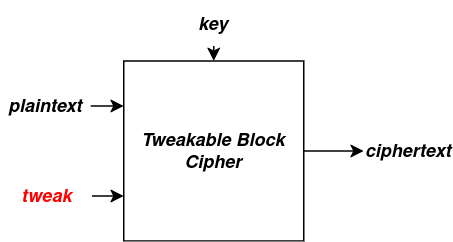
\includegraphics[width=0.45\textwidth]{img/tweak_bd.png}
        \par}

        \item \textcolor{red}{\textbf{\textit{Xor Encrypt Xor - XEX}}} è una progettazione standard per costruire un \textit{tweakable cipher} basandosi su un \textit{block cipher} standard, garantendo \textbf{\textit{length-preserving}} accetta in input dati che abbiano dimensione multipla della \textit{block size}. \textbf{XEX} necessita di \textbf{due chiavi distinte}, che possono essere derivate o estese dalla stessa dal \textit{layer} sopra.

        \begin{figure}[h]
            \centering
            \begin{minipage}[c]{0.45\textwidth}
                \centering
                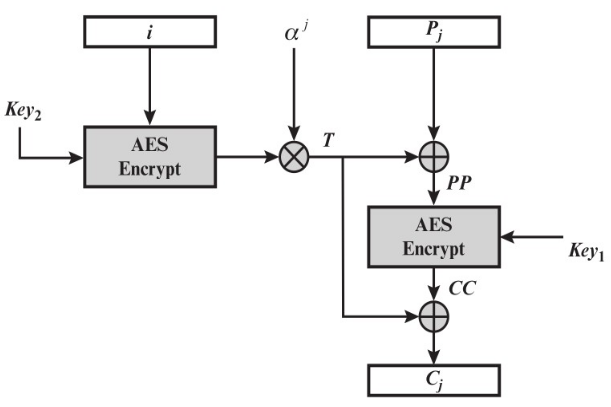
\includegraphics[width=\textwidth]{img/xex_enc.png}
                \caption{XEX Encryption}
            \end{minipage}
            \hfill
            \begin{minipage}[c]{0.45\textwidth}
                \centering
                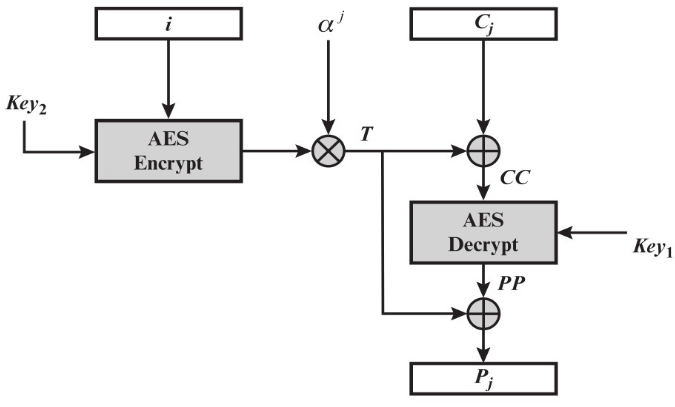
\includegraphics[width=\textwidth]{img/xex_dec.png}
                \caption{XEX Decryption}
            \end{minipage}
        \end{figure}
        
        \item \textcolor{red}{\textbf{\textit{Ciphertext Stealing - CTS}}}: è una tecnica utilizzata per supportare dati di lunghezza variabile negli schemi di cifratura a blocchi, tuttavia introduce un stretta dipendenza tra gli ultimi due blocchi, a volte è stata anche utilizzare per mitigare gli attacchi legati al \textit{padding oracle}, oggi si preferisce la cifratura autenticata.

        \begin{figure}[h]
            \centering
            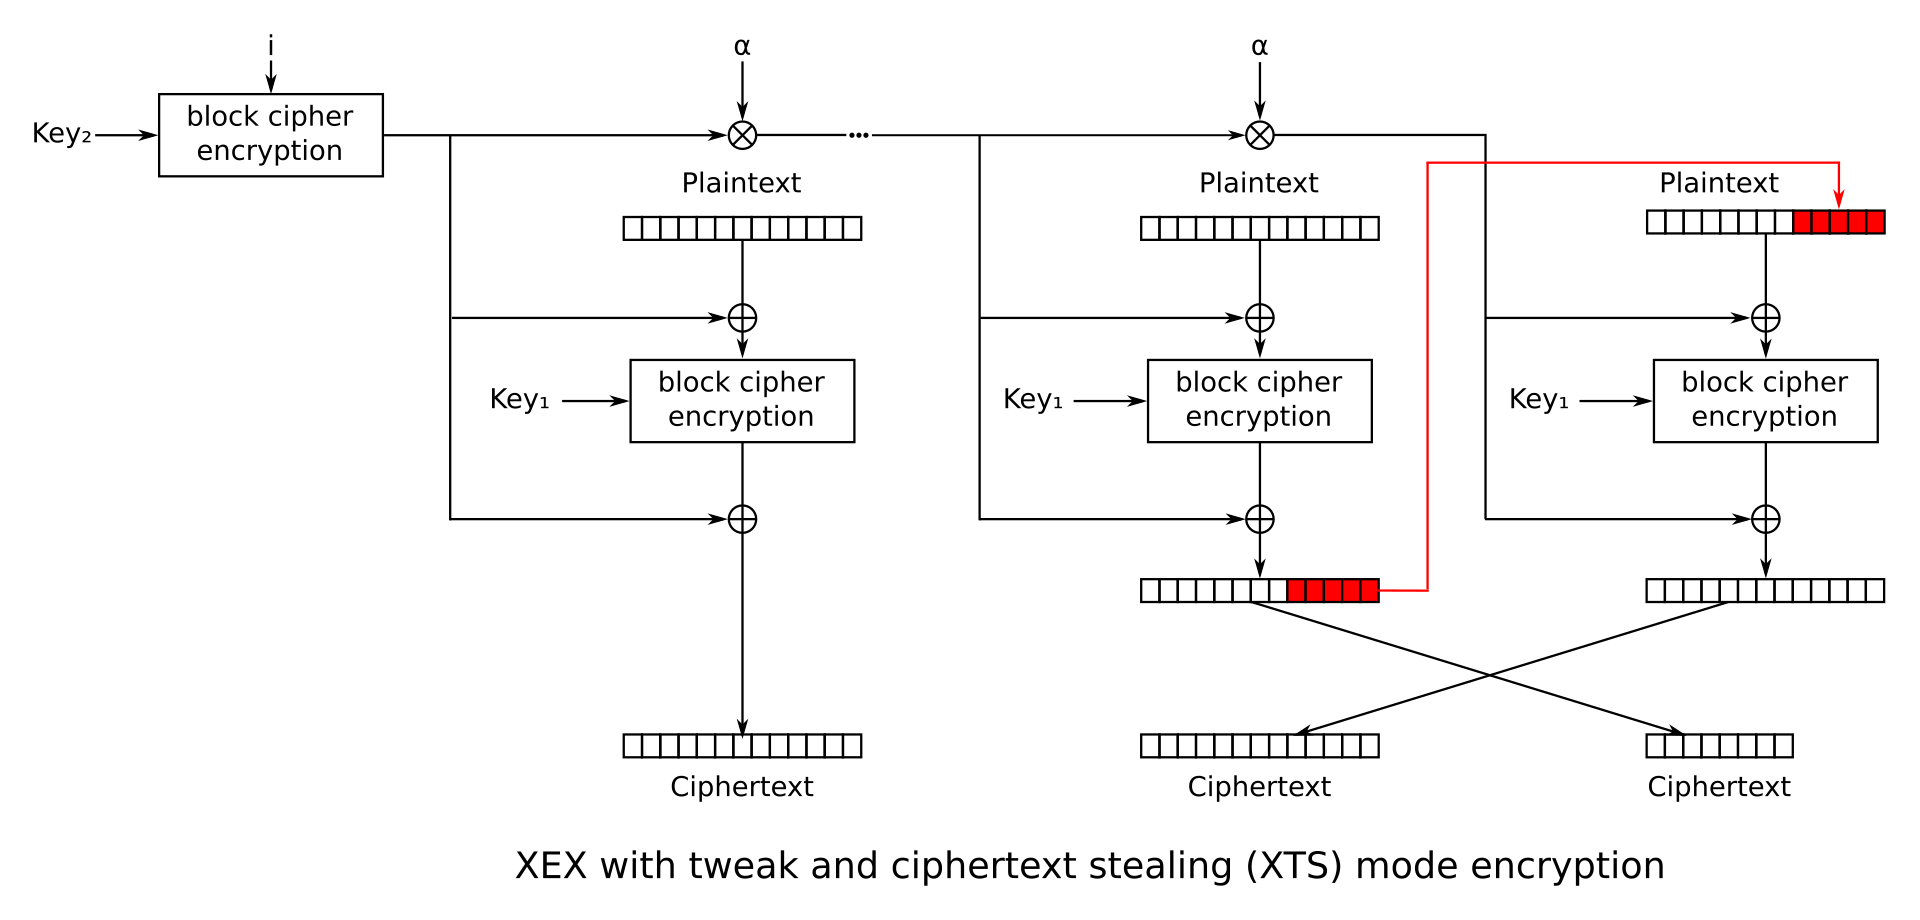
\includegraphics[width=\textwidth]{img/xts.png}
            \caption{XTS Encryption}
        \end{figure}
    \end{itemize}
\end{flushleft}

\section{Wide Block Encryption}
\begin{flushleft}
    Un blocco \textbf{\textit{wide encryption}} è modellato per la cifratura di \textit{disk sector} ed è rappresentabile come un \textbf{\textit{Super Pseudo Random Permutation}} che accetta come parametri:
    \begin{itemize}[nosep]
        \item un \textbf{\textit{tweak}} per supportare la randomizzazione basata sulla locazione dell'informazione.
        \item una \textbf{\textit{block size}} che regola la quantità di dati che è contenuta nella permutazione.
    \end{itemize}
    È basato su un \textit{block cipher} con una dimensione ridotta e fissa.

    \begin{figure}[h]
        \centering
        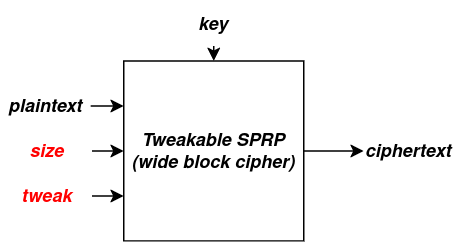
\includegraphics[width=0.45\textwidth]{img/wide_block.png}
    \end{figure}
\end{flushleft}